\documentclass{article}
\usepackage{amsmath,amssymb,setspace,verbatim,graphicx,enumerate,enumitem}
\usepackage[top=1in,bottom=1in,left=1in,right=1in,head=0.5in,foot=0.5in]{geometry}
\usepackage{caption}
\usepackage{mathtools}
% \usepackage{subcaption}
% \usepackage{subfig}
% \usepackage{subfloat}
% \usepackage{tabularx}
\usepackage{mdframed}
\usepackage{amsthm}

\newtheorem*{theorem}{Theorem}

\newenvironment{Rcode}% environment name 
{%begin code
    \begin{mdframed}
    \#R code
    \begin{small}
}
{%end code
    \end{small}
    \end{mdframed}
}

\newenvironment{console}% environment name 
{%begin code
    \begin{mdframed}
    \#Console
    \begin{small}
}
{%end code
    \end{small}
    \end{mdframed}
}

\begin{document}
\title{STDA Homework 3}
\author{Seokjun Choi}
\date{June 3, 2020}
\maketitle

\textbf{Note:}
Sorry for being delayed. 

\textbf{Note:}
You can get full code files at my github page: Visit https://github.com/letsjdosth/SpaTempoDA \\
and see "HW3" directory. Because I provide the full code separately, in this report 
I will show key code blocks only, instead of the whole, verbose code.

\section{Problem}
\textbf{
Analyze data on rental rates in Munich.
}
\subsection{OLS fit}

In the beginning, I fit the given data to a linear model using least squares, 
without considering spatial correlation. In detail, the model is specified by
\begin{align*}
RentPermM2 = \beta_1 + \beta_2 Year + \beta_3 NoHotWater + \beta_4 NoCentralHeat \\
+ \beta_5 NoBathTiles + \beta_6 SpecialBathroom + \beta_7 SpecialKitchen\\
+ \beta_8 Room2 + \beta_9 Room3 + \beta_10 Room4 + \beta_11 Room5 + \beta_12 Room6 + \epsilon
\end{align*}
where $\epsilon \sim N(0,\sigma^2)$.

(For coherence to the notation of bayesian model below and to the variable names of code,
I denote the intercept term as $\beta_1$, although the convention is $\beta_0$.)

Using "lm" function on R, get the result of fitting. This is a part of summary.

\begin{verbatim}
Coefficients:
                  Estimate Std. Error t value Pr(>|t|)
(Intercept)     -16.012330   4.048974  -3.955 7.93e-05 ***
Year              0.013331   0.002059   6.473 1.20e-10 ***
NoHotWater       -1.870505   0.303264  -6.168 8.33e-10 ***
NoCentralHeat    -1.225761   0.206737  -5.929 3.57e-09 ***
NoBathTiles      -0.725711   0.123431  -5.879 4.80e-09 ***
SpecialBathroom   0.660372   0.169562   3.895 0.000102 ***
SpecialKitchen    1.462887   0.185429   7.889 4.94e-15 ***
Room2            -1.319372   0.157060  -8.400  < 2e-16 ***
Room3            -1.886408   0.156998 -12.016  < 2e-16 ***
Room4            -2.464631   0.193683 -12.725  < 2e-16 ***
Room5            -2.378158   0.343380  -6.926 5.80e-12 ***
Room6            -2.482621   0.590678  -4.203 2.75e-05 ***
---
Signif. codes:  0 '***' 0.001 '**' 0.01 '*' 0.05 '.' 0.1 ' ' 1
\end{verbatim}

When considering the context which the data were generated, however,
the data may have spatial correlation. If so,
the above model and fitting result are invalid, because it neglects the spatial consideration.


\clearpage
\subsection{EDA}
Now, see given data with the map of Munich. There are 380 districts in the city, and
among the districts, some are just field or park, having no apartments. I mark the
districts as 'grey' color on the below map.

\begin{figure}[!h]
    \centering
    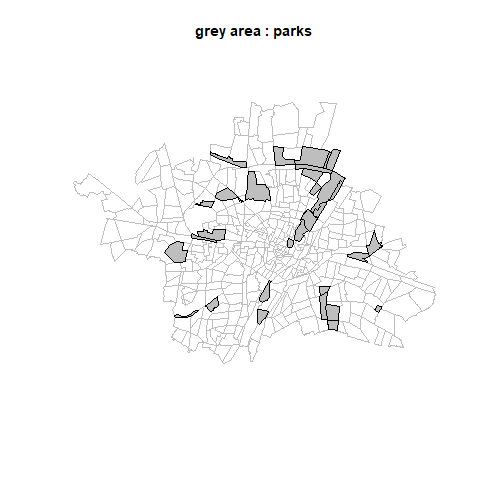
\includegraphics[width=7cm]{map_parks.png}
    \caption{Districts map of Munich. \\ Gray area : park or field. (No apartments)}
\end{figure}

I set a neighborhood structure. If two districts share a common boundary,
then I define two districts are neighbor. The left plot of below is the result of applying this rule.

In addition, the given dataset has 2035 observations, and each one has the location information
where the apartment is. The right plot of below is the map indicating the number of observations for each district.

\begin{figure}[!h]
    \centering
    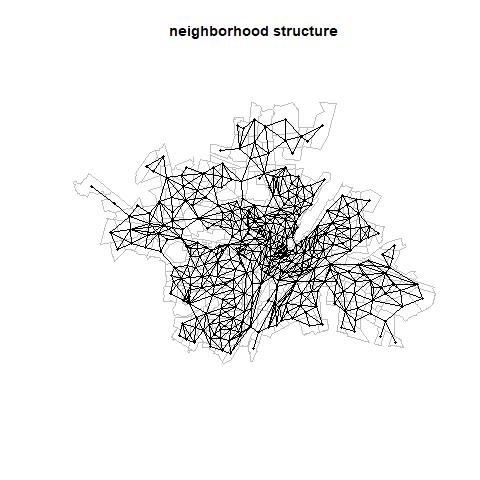
\includegraphics[width=7cm]{map_neighborhood_structure.png}
    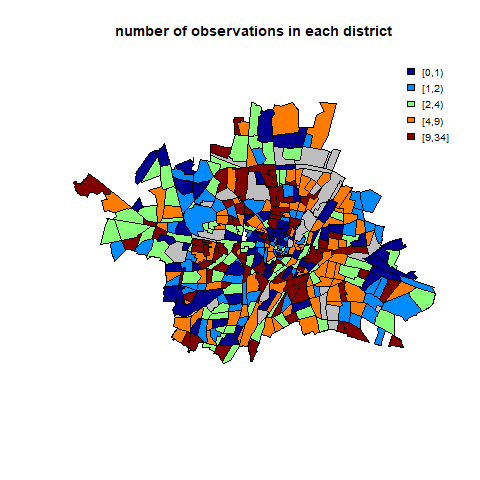
\includegraphics[width=7cm]{map_obsnum.png}
    \caption{left : The neighborhood structure defined by shared boundary.
    \\right: the number of observations for each district. (gray: park or field)}
\end{figure}



\clearpage
\subsection{Analysis: Bayesian approach}
In this subsection, I will construct a Bayesian model 
to considering spatial correlation which the data may have.

Set a hierarchical model as belows. \\
Data:
\[Y|\beta,\eta,\sigma^2 \sim MVN(X\beta+H\eta, \sigma^2I)\]
Process:
\[p(\eta|\tau^2) \propto (\tau^2)^{-(m-1)/2} exp{(-\frac{1}{2\tau^2}\eta'(D_w-W)\eta)}\]
Prior:
\[p(\beta)\propto 1 , \sigma^2,\tau^2 \sim InverseGamma(0.001, 0.001)\]
where $X$: variables of data with column of 1, $W$: neighborhood structure matrix(binary), H:mapping between the districts (of order in districts.sp) and rents data,
and $D_w$: diagonal matrix with elements made by row sums of $W$.
Note that, the $X\beta$ term in the data model is correspond to a 'trend' with covariant factors, like
\begin{align*}
    RentPermM2 = \beta_1 + \beta_2 Year + \beta_3 NoHotWater + \beta_4 NoCentralHeat \\
    + \beta_5 NoBathTiles + \beta_6 SpecialBathroom + \beta_7 SpecialKitchen\\
    + \beta_8 Room2 + \beta_9 Room3 + \beta_10 Room4 + \beta_11 Room5 + \beta_12 Room6
\end{align*}
(I denote the intercept term as $\beta_1$, although the convention is $\beta_0$.)
and the $H\eta$ term in the data model and the process model catches a spatial covariance structure of data.

And also note that, this model is a form of "intrinsic auto-regressive model" so that getting full conditional distributions is easy.
Thus, using the Gibbs sampler, I will get posterior samples of the model and analyze the data.

The key parts of an implementation of the Gibbs sampler are here. 
I set the initial condition arbitrary (see the list named "gibbs.initial\_cond" in the code), 
and the number of iteration 10,000.

\begin{Rcode}
    \begin{verbatim}
## gibbs sampler
# creating model matrix
# help(nb2mat)
model.W = nb2mat(nb.bound, style="B")
model.Dw = diag(x = rowSums(model.W), 380, 380)

model.H = H
model.m = dim(H)[2] #380
model.n = length(y) #2035
        
# Full conditional distributions
# calculate some expensive matrix
model.inv.tXX = solve(t(X)%*%X)
model.tHH = t(model.H)%*%model.H
model.Dw_minus_W = model.Dw-model.W

#beta
gibbs.cond.beta = function(last_param){
    cond.mean = model.inv.tXX %*% t(X) %*% (y - model.H %*% last_param$eta)
    cond.var = last_param$sigma2 * model.inv.tXX
    new_beta = rmvnorm(1, mean=cond.mean, sigma=cond.var)
    return(new_beta)
}

gibbs.cond.eta = function(last_param){
    cond.precision = (1/last_param$sigma2) * model.tHH + (1/last_param$tau2) * model.Dw_minus_W
    cond.var = solve(cond.precision)
    cond.mean = (1/last_param$sigma2)*cond.var %*% t(model.H) %*% (y - X%*%last_param$beta)
    new_eta = rmvnorm(1, mean=cond.mean, sigma=cond.var)
    new_eta = new_eta - mean(new_eta) # imposing constraint
    return(new_eta)
}

gibbs.cond.sigma2 = function(last_param){
    cond.shape = 0.001 + model.n/2
    diff_fit = y - X%*%last_param$beta - model.H%*%last_param$eta
    cond.scale = 0.001 + 0.5 * t(diff_fit) %*% diff_fit
    new_sigma2 = rinvgamma(1, shape=cond.shape, scale=cond.scale)
    return(new_sigma2)
}

gibbs.cond.tau2 = function(last_param){
    cond.shape = 0.001 + (model.m - 1)/2
    cond.scale = 0.001 + 0.5 * t(last_param$eta) %*% model.Dw_minus_W %*% last_param$eta
    new_tau2 = rinvgamma(1, shape=cond.shape, scale=cond.scale)
    return(new_tau2)
}

# sampler
gibbs.iter.B = 10000
gibbs.param_mat = matrix(0, gibbs.iter.B, 12+380+1+1) # order: beta, eta, sigma2, tau2

gibbs.initial_cond = list(
    beta = c(rnorm(12,0,1)), #dim 12
    eta = c(rnorm(380,0,10)), #dim 380
    sigma2 = 1, #dim 1
    tau2 = 1 #dim 1
)

gibbs.last_param = gibbs.initial_cond
gibbs.param_mat[1,]=unlist(gibbs.last_param)

gibbs.start_time = Sys.time()
print("gibbs: start sampling")
for(i in 2:gibbs.iter.B){
    if(i%%20==0) {
        elapsed = Sys.time()-gibbs.start_time
        est_time_total = elapsed * gibbs.iter.B / i
        est_time_remain = est_time_total - elapsed
        cat("iteration: ", i,"/",gibbs.iter.B,", remain(estimated):", est_time_remain,"\n")
    }
    gibbs.last_param$beta = c(gibbs.cond.beta(gibbs.last_param))
    gibbs.last_param$eta = c(gibbs.cond.eta(gibbs.last_param))
    gibbs.last_param$sigma2 = c(gibbs.cond.sigma2(gibbs.last_param))
    gibbs.last_param$tau2 = c(gibbs.cond.tau2(gibbs.last_param))
    gibbs.param_mat[i,] = unlist(gibbs.last_param)
}
print("gibbs: end sampling")
gibbs.end_time = Sys.time()
cat("gibbs: execution time: ", gibbs.end_time-gibbs.start_time, "\n")
    \end{verbatim}
\end{Rcode}

The execution time is about 35 minutes on my computer.

After generating them, I cut the first 1000 samples as burn-in period and doesn't do thinning.
As a result, I report histograms, traceplots, and acf plots for each variable except $\eta$.
(Order: $\beta_1 \sim \beta_{12}$,$\sigma^2$,$\tau^2$)


\begin{figure}[!h]
    \centering
    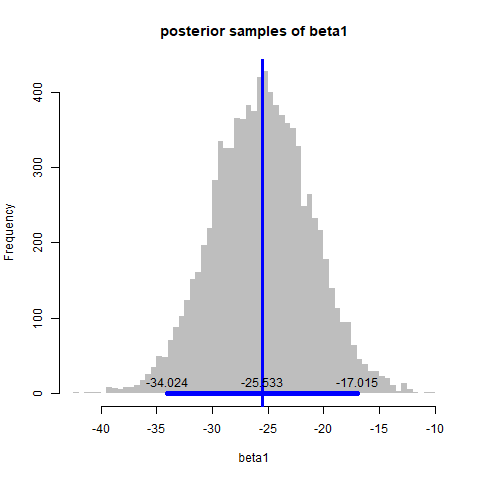
\includegraphics[width=4cm]{beta1_hist.png}
    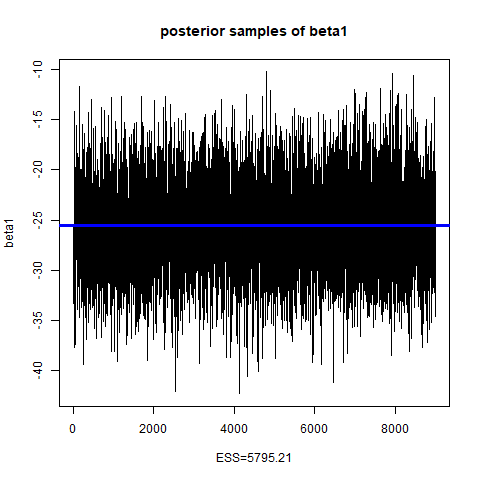
\includegraphics[width=4cm]{beta1_traceplot.png}
    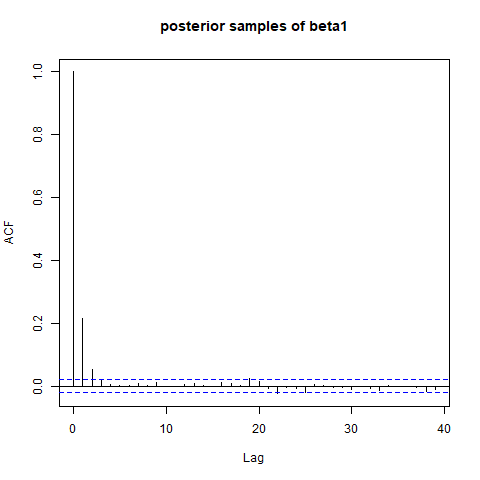
\includegraphics[width=4cm]{beta1_acf.png} \\
    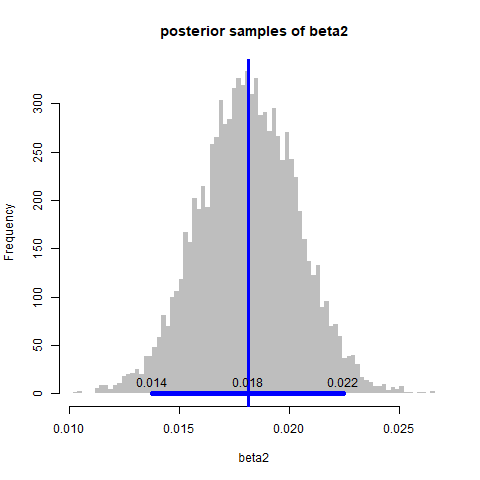
\includegraphics[width=4cm]{beta2_hist.png}
    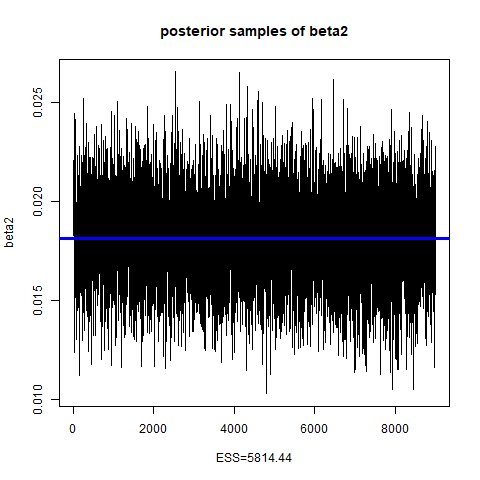
\includegraphics[width=4cm]{beta2_traceplot.png}
    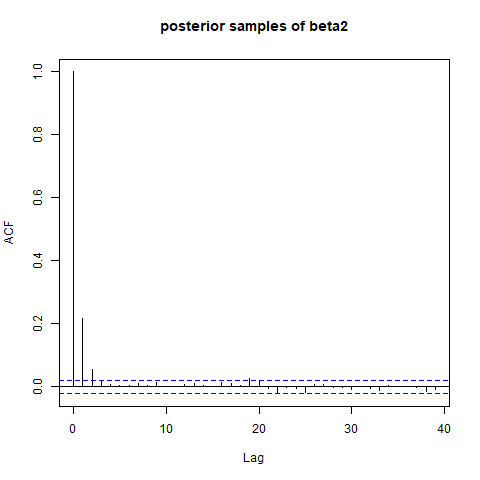
\includegraphics[width=4cm]{beta2_acf.png} \\
    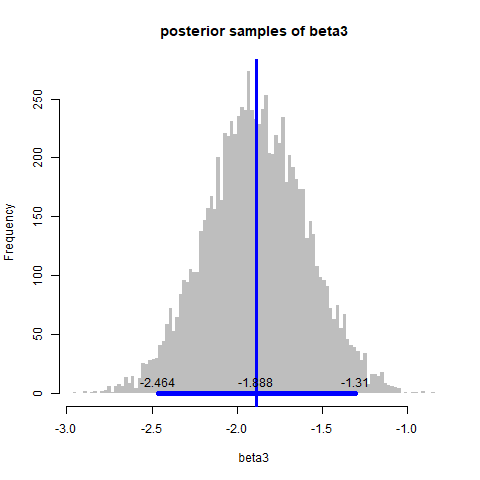
\includegraphics[width=4cm]{beta3_hist.png}
    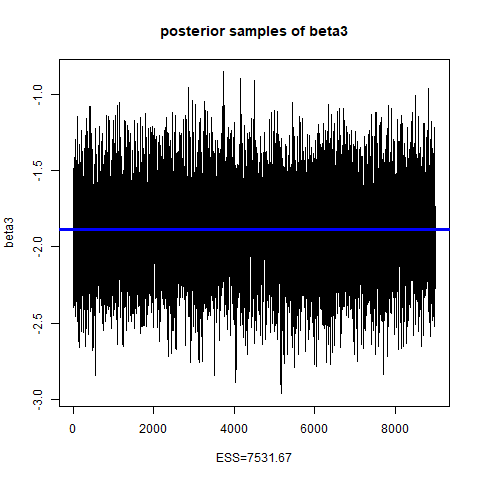
\includegraphics[width=4cm]{beta3_traceplot.png}
    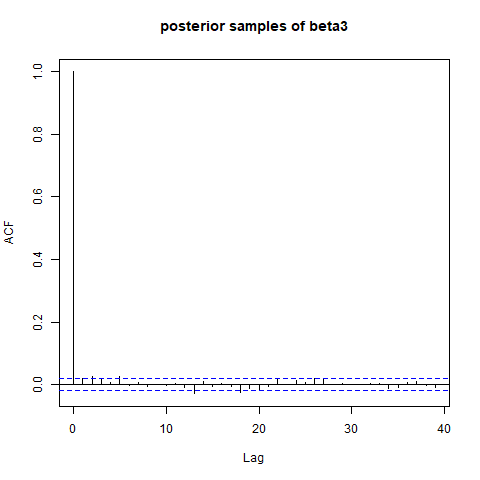
\includegraphics[width=4cm]{beta3_acf.png} \\
    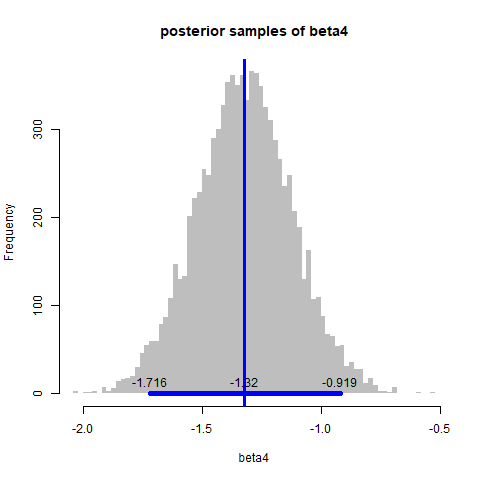
\includegraphics[width=4cm]{beta4_hist.png}
    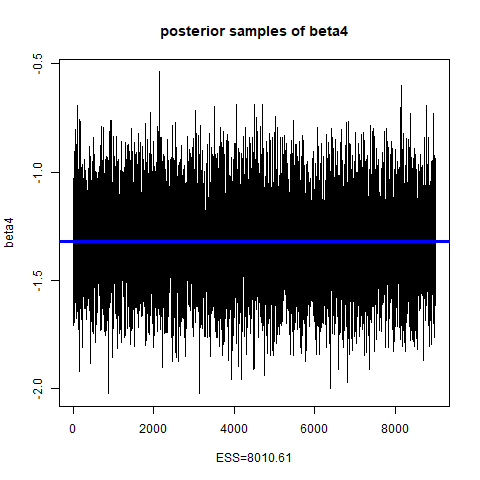
\includegraphics[width=4cm]{beta4_traceplot.png}
    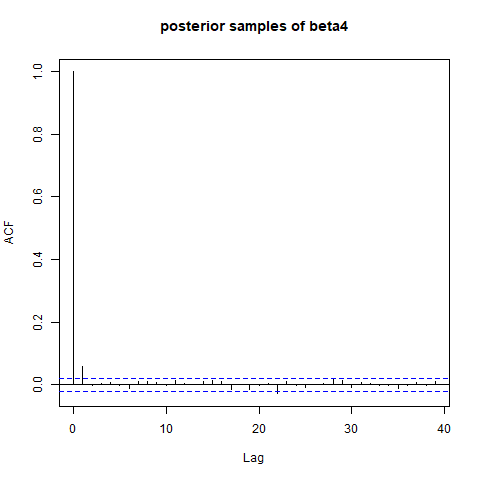
\includegraphics[width=4cm]{beta4_acf.png} \\
    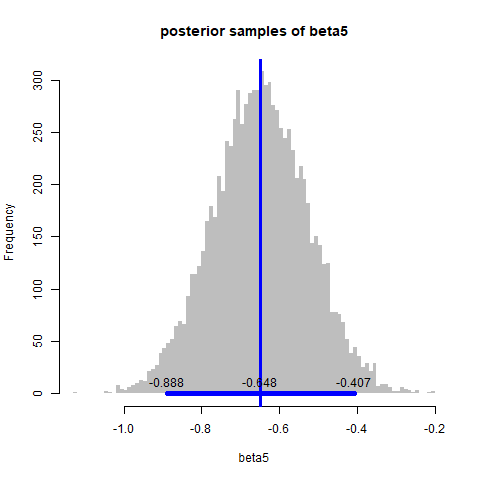
\includegraphics[width=4cm]{beta5_hist.png}
    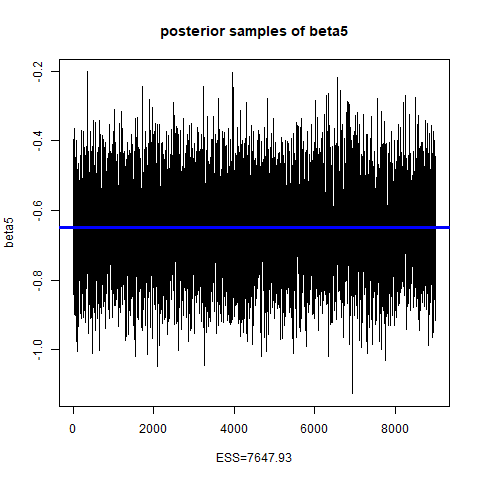
\includegraphics[width=4cm]{beta5_traceplot.png}
    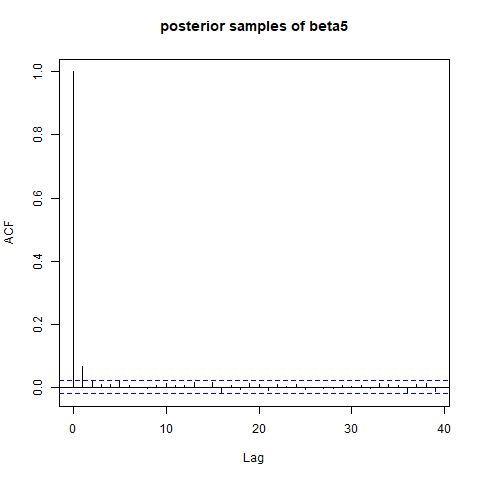
\includegraphics[width=4cm]{beta5_acf.png}
    \caption{For each parameter, \\left: histogram, mean, 95\% credible interval of posterior samples, mid: traceplot and ESS, right:acf plot}
\end{figure}
\begin{figure}[!h]
    \centering
    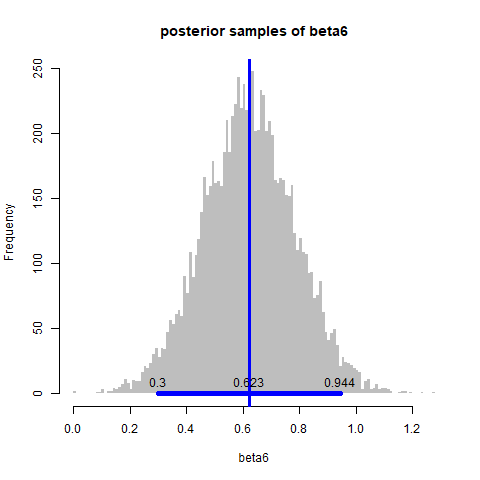
\includegraphics[width=4cm]{beta6_hist.png}
    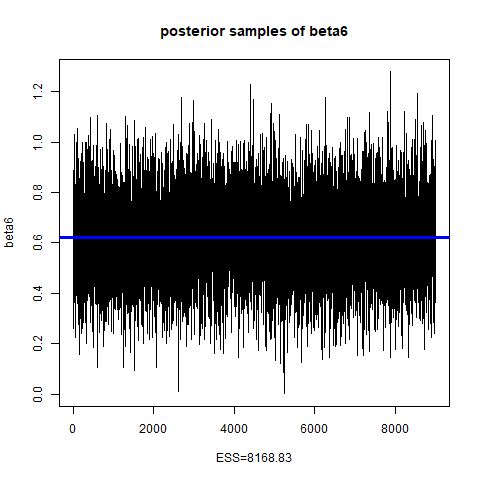
\includegraphics[width=4cm]{beta6_traceplot.png}
    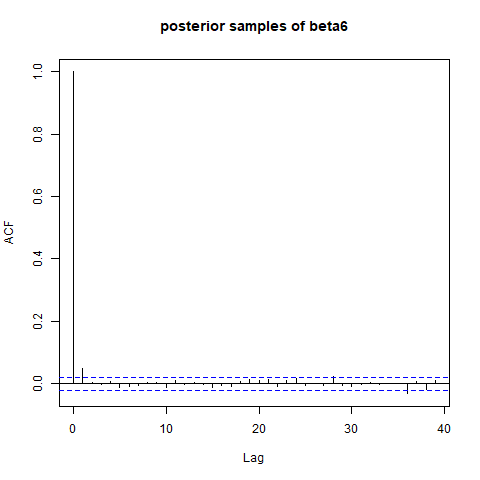
\includegraphics[width=4cm]{beta6_acf.png} \\
    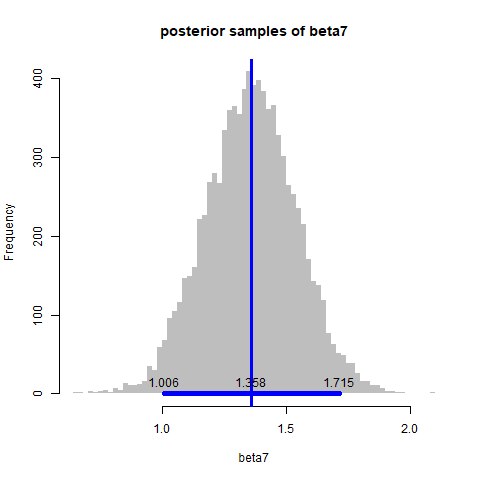
\includegraphics[width=4cm]{beta7_hist.png}
    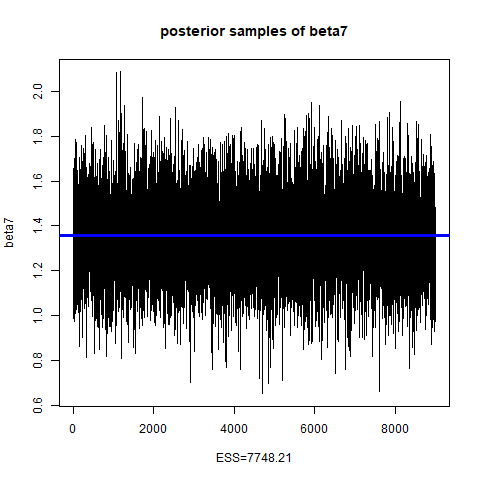
\includegraphics[width=4cm]{beta7_traceplot.png}
    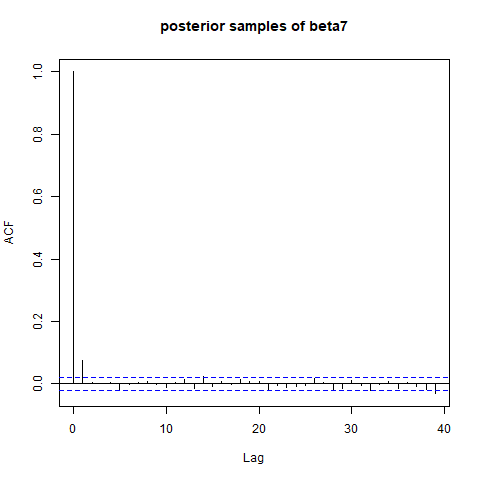
\includegraphics[width=4cm]{beta7_acf.png} \\
    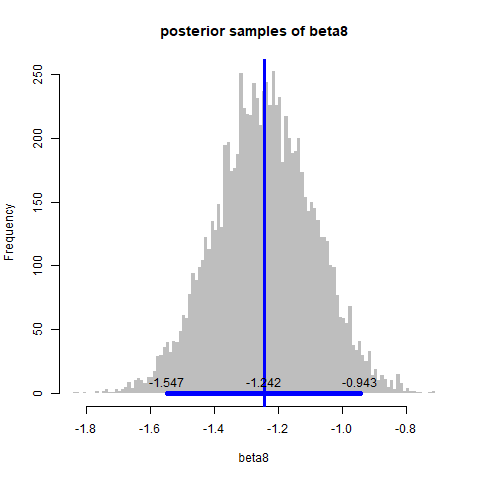
\includegraphics[width=4cm]{beta8_hist.png}
    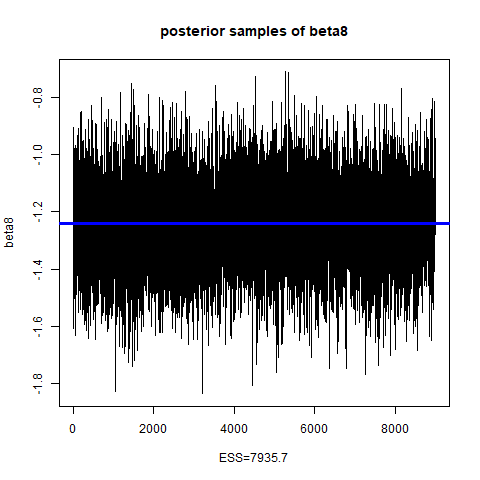
\includegraphics[width=4cm]{beta8_traceplot.png}
    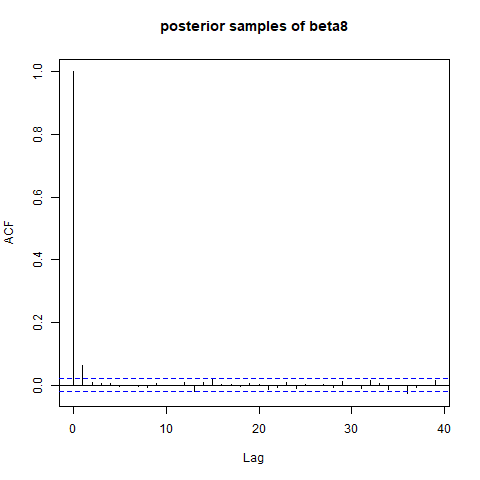
\includegraphics[width=4cm]{beta8_acf.png} \\
    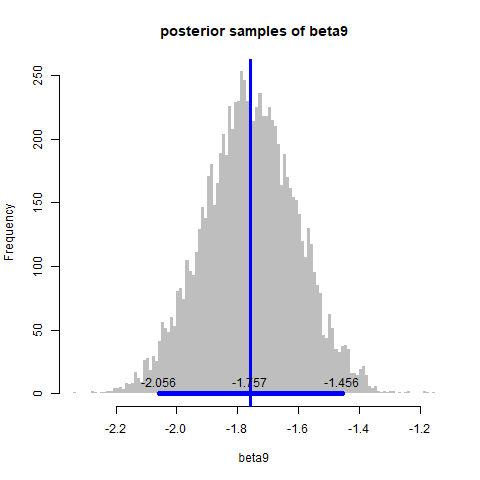
\includegraphics[width=4cm]{beta9_hist.png}
    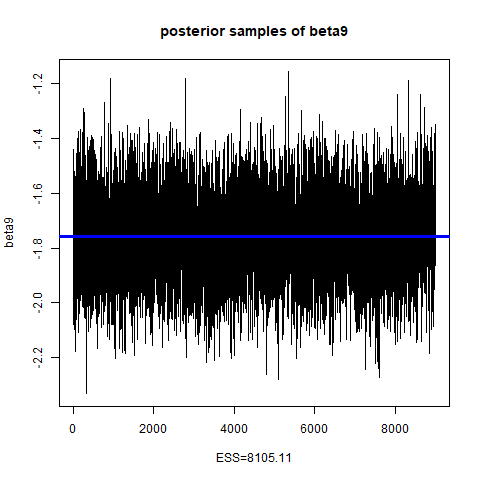
\includegraphics[width=4cm]{beta9_traceplot.png}
    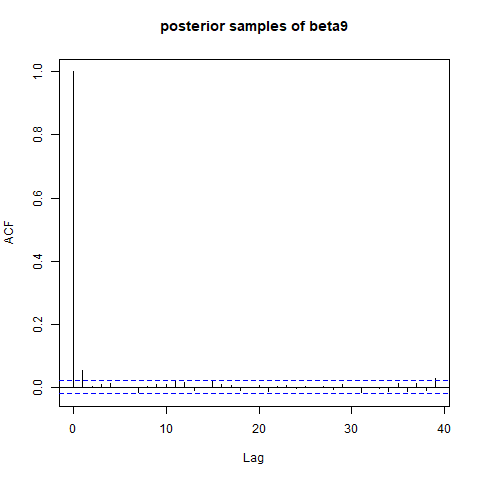
\includegraphics[width=4cm]{beta9_acf.png} \\
    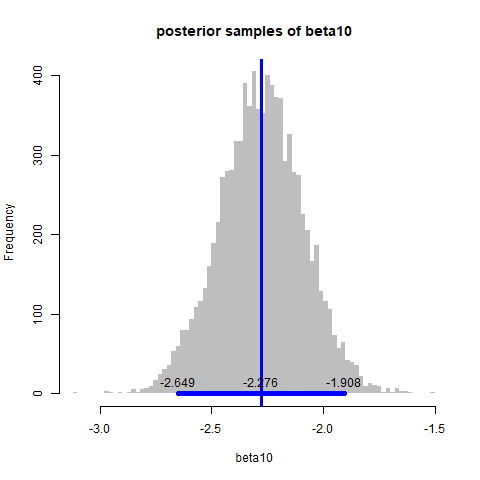
\includegraphics[width=4cm]{beta10_hist.png}
    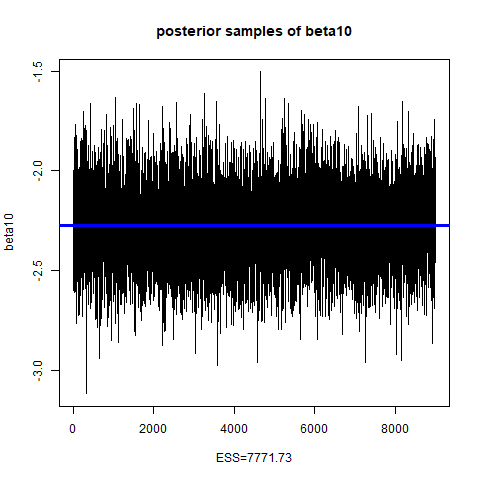
\includegraphics[width=4cm]{beta10_traceplot.png}
    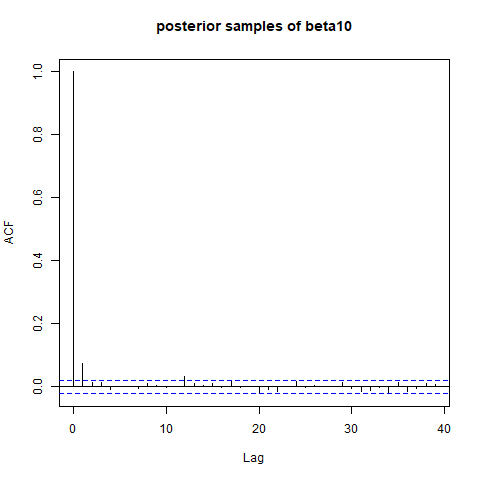
\includegraphics[width=4cm]{beta10_acf.png}
    \caption{For each parameter, \\left: histogram, mean, 95\% credible interval of posterior samples, mid: traceplot and ESS, right:acf plot}
\end{figure}
\begin{figure}[!h]
    \centering
    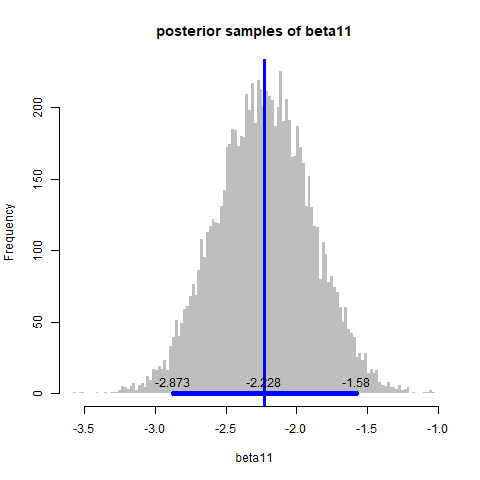
\includegraphics[width=4cm]{beta11_hist.png}
    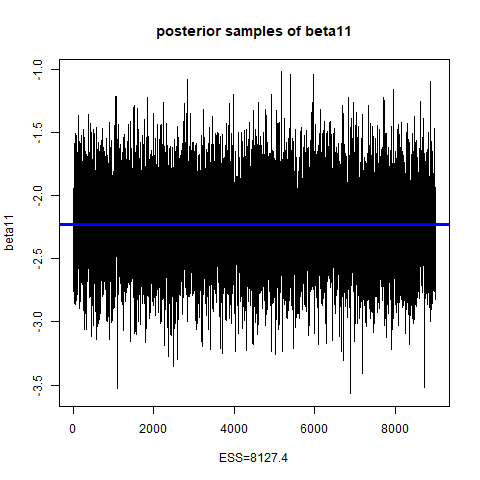
\includegraphics[width=4cm]{beta11_traceplot.png}
    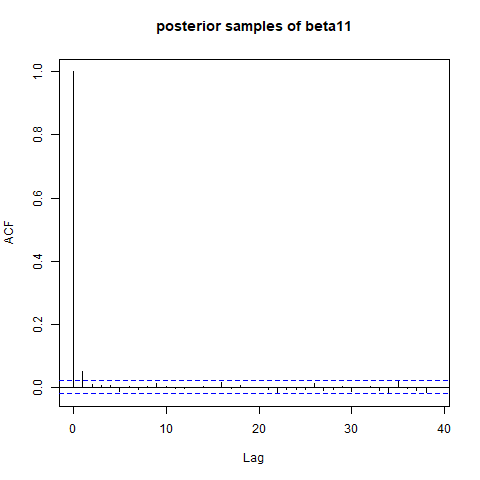
\includegraphics[width=4cm]{beta11_acf.png} \\
    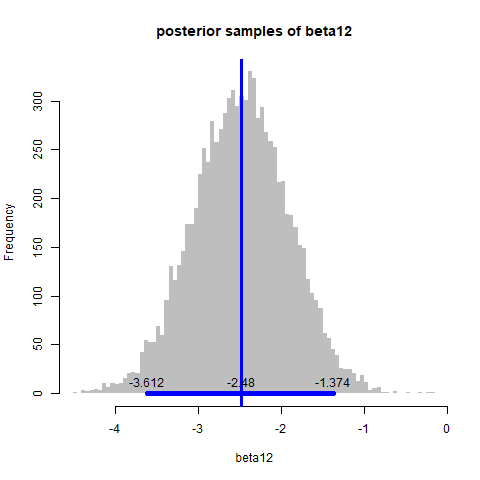
\includegraphics[width=4cm]{beta12_hist.png}
    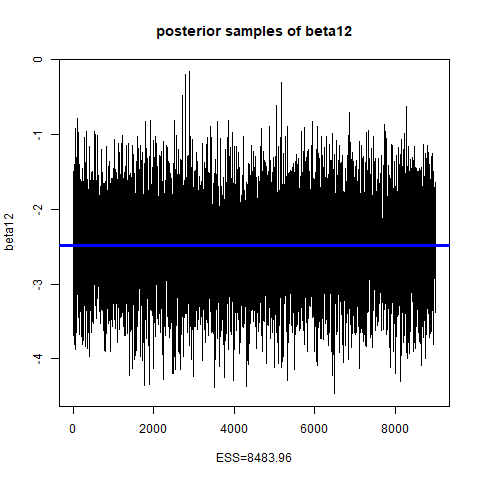
\includegraphics[width=4cm]{beta12_traceplot.png}
    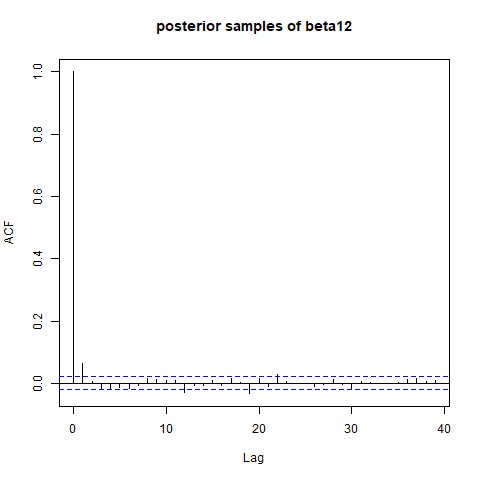
\includegraphics[width=4cm]{beta12_acf.png} \\
    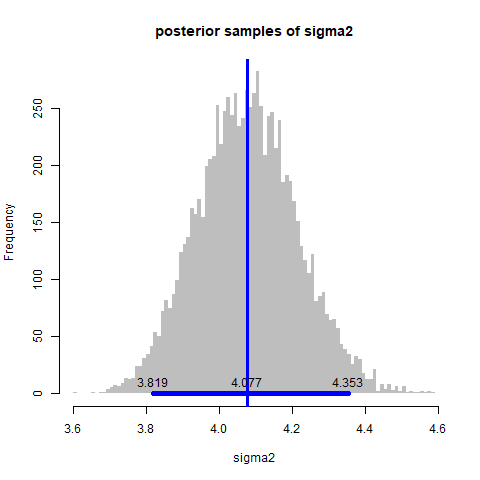
\includegraphics[width=4cm]{sigma2_hist.png}
    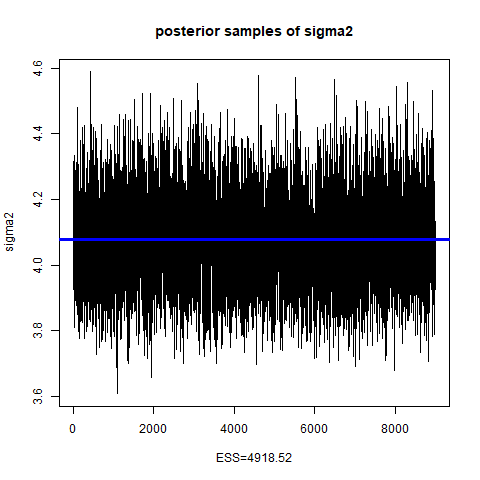
\includegraphics[width=4cm]{sigma2_traceplot.png}
    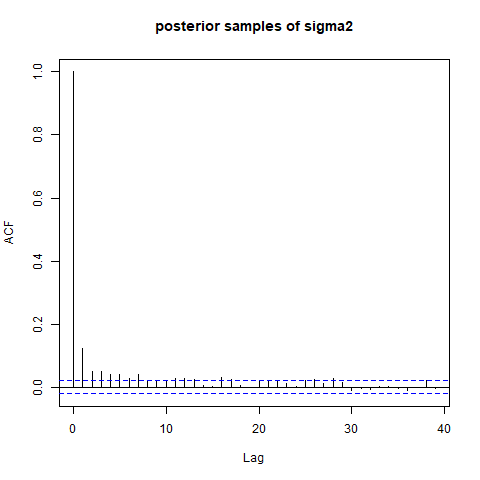
\includegraphics[width=4cm]{sigma2_acf.png} \\
    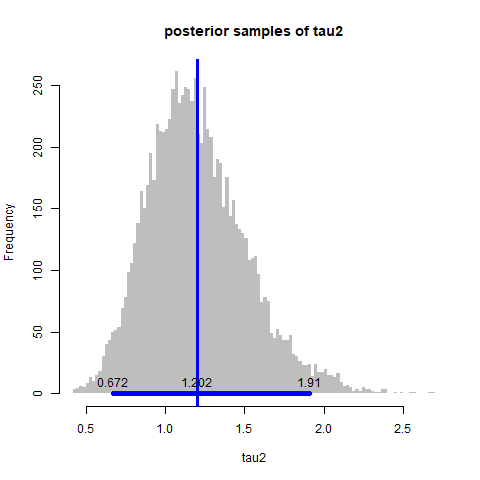
\includegraphics[width=4cm]{tau2_hist.png}
    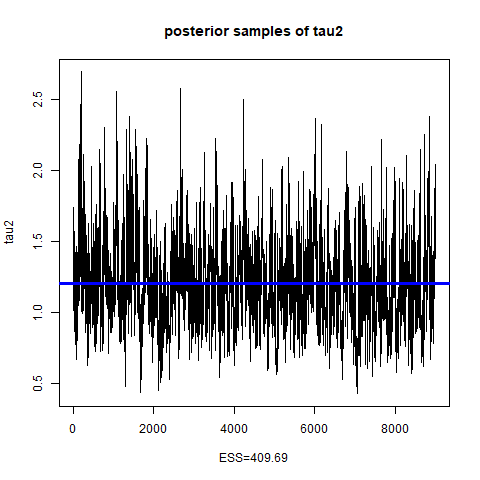
\includegraphics[width=4cm]{tau2_traceplot.png}
    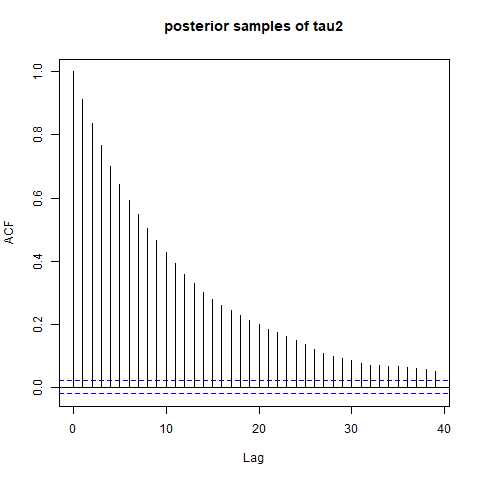
\includegraphics[width=4cm]{tau2_acf.png}
    \caption{For each parameter, \\left: histogram, mean, 95\% credible interval of posterior samples, mid: traceplot and ESS, right:acf plot}
\end{figure}

\clearpage
Note that last two rows are plots of $\sigma^2$, $\tau^2$, respectively.
Except the samples of $\tau^2$, samples of all parameters are generated quite well.

Commonly, the variance parameters have high correlation, and the $\tau^2$ of our model also has same problem.
So the ESS of $\tau^2$ is lower than other parameter's, and the acf also vanishes slower. 
If you want deal with the autocorrelation, you may run more iterations and do thinning.

As a summary, here is the table of sample mean and 95\% credible interval of all parameters except $\eta$.
\begin{verbatim}
          mean  0.025q  0.975q
beta1  -25.533 -34.024 -17.015
beta2    0.018   0.014   0.022
beta3   -1.888  -2.464  -1.310
beta4   -1.320  -1.716  -0.919
beta5   -0.648  -0.888  -0.407
beta6    0.623   0.300   0.944
beta7    1.358   1.006   1.715
beta8   -1.242  -1.547  -0.943
beta9   -1.757  -2.056  -1.456
beta10  -2.276  -2.649  -1.908
beta11  -2.228  -2.873  -1.580
beta12  -2.480  -3.612  -1.374
sigma^2  4.077   3.819   4.353
tau^2    1.202   0.672   1.910
\end{verbatim}

For summarizing $\eta$, I report the map of posterior means and standard deviations for each $\eta_s$.
($s=1,2,...,380$)
\begin{figure}[!h]
    \centering
    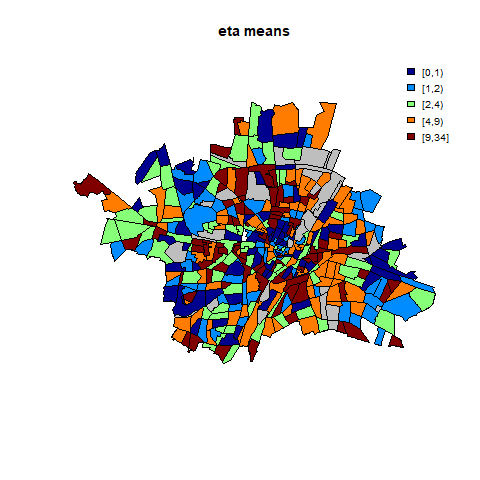
\includegraphics[width=7cm]{map_posterior_eta_means.png}
    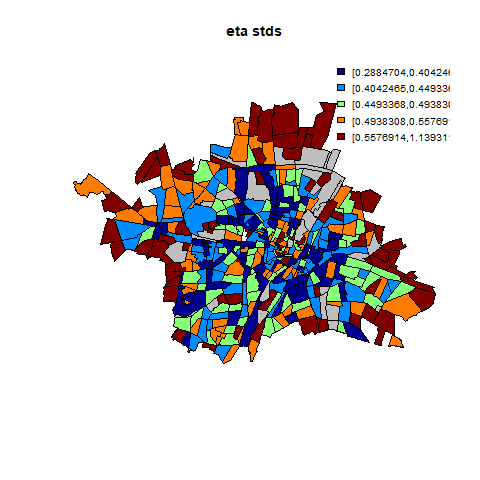
\includegraphics[width=7cm]{map_posterior_eta_stds.png}
    \caption{mean(left) and standard deviation(right) of posterior samples of $\eta$}
\end{figure}

On the posterior mean plot, it is seen that some clusters of lower or higher mean values exist.
The center region has relatively low $\eta$ value, and circle-shaped region surrounding the center region has quite high value of $\eta$.
And, the marginal regions of north-west and south-east have low $eta$ value.
Hence, I can conclude that some spatial correlations exists, and the Bayesian hierarchical model catch the correlation properly.

Also, the standard deviations are low in the districts which have many neighbors (like the center region), and 
high in the districts which have fewer neighbors (like the region of boundary). It is a natural property of spatial model.
So I can draw a conclusion that our fitting is done well.

\end{document}